\documentclass[10pt]{article}

\usepackage[english]{babel}
\usepackage[utf8x]{inputenc}
\usepackage{amsmath}
\usepackage{amssymb}
\usepackage{amsfonts}
\usepackage{graphicx}
\usepackage[ruled,linesnumbered,noend]{algorithm2e}
\usepackage{empheq}
\usepackage{float}
\usepackage{enumitem}
\usepackage{tikz}
\usepackage[colorlinks=true,urlcolor=blue]{hyperref}

\title{Introduction to Machine Learning, Fall 2015 - Exercise session VI}
\author{Rodion ``rodde'' Efremov, student ID 013593012}

\begin{document}
 \maketitle

\section*{Intro}
The only material I used are the slides. Did not discuss in a group, except mailed Amin about possible ``typo'' which wasn't one. I omitted the pen and paper exercises.

\section{Problem 4 (Programming task)}
\subsection{k-means}
\subsubsection{Uset first 10 images as the initial cluster means}
So when I run the $k$-means algorithm using \textbf{10 first images} as the initial means, I get the following means:
\begin{figure}
\begin{center}
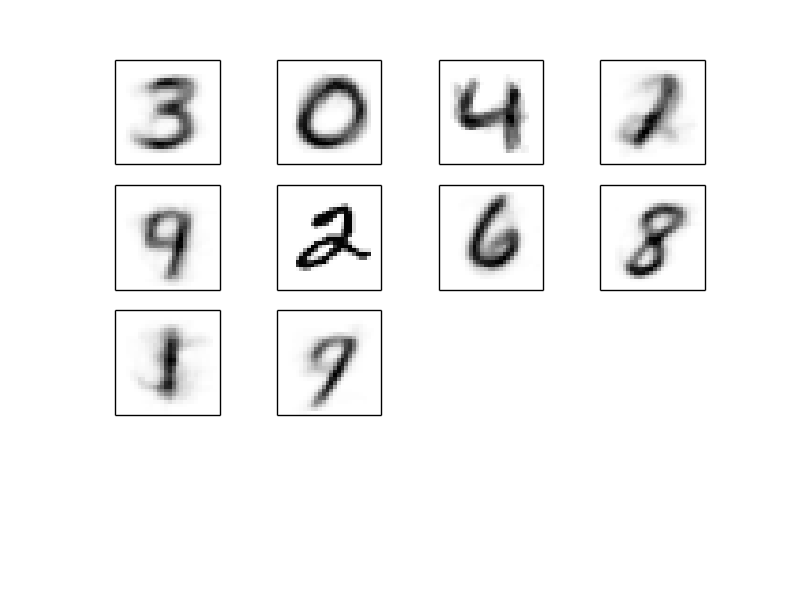
\includegraphics[scale=0.5]{meansA}
\caption{First iteration cluster means}
\end{center}
\end{figure}
And the classified digits follow:
\begin{figure}
\begin{center}
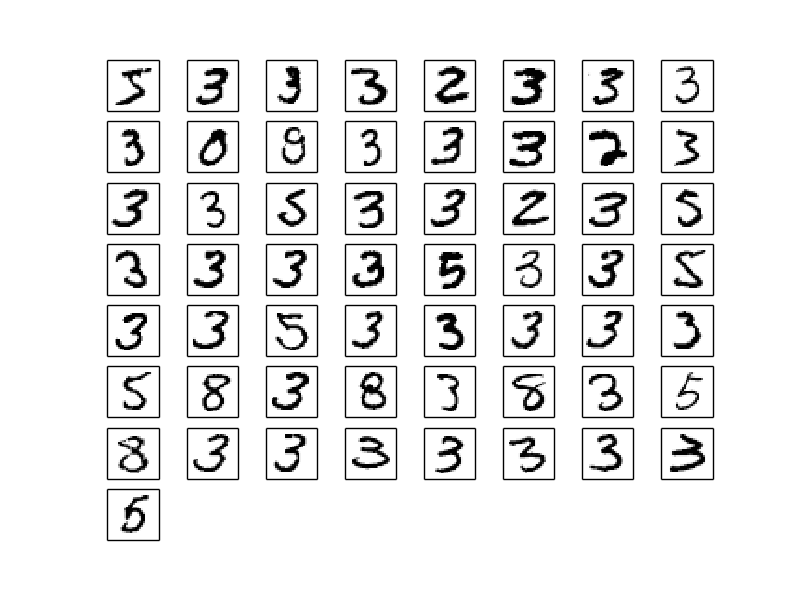
\includegraphics[scale=0.5]{meansA0}
\caption{Digits 0}
\end{center}
\end{figure}
\begin{figure}
\begin{center}
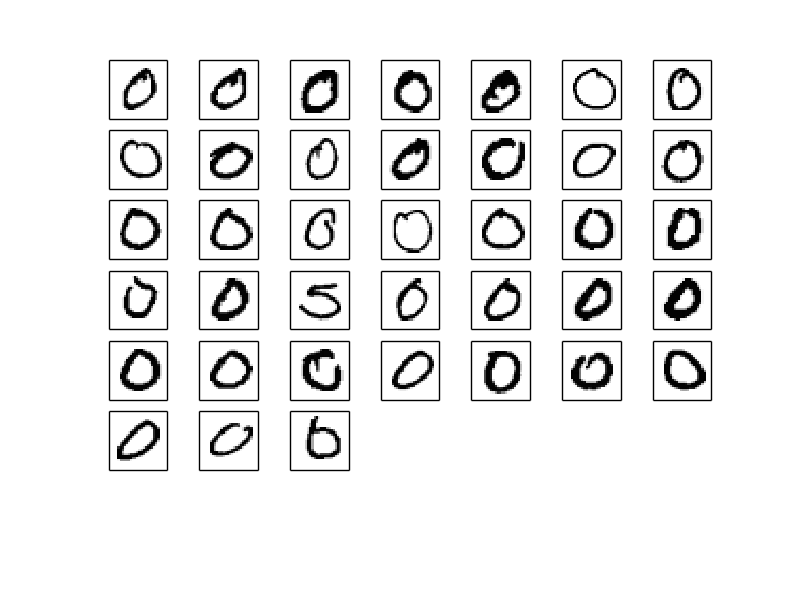
\includegraphics[scale=0.5]{meansA1}
\caption{Digits 1}
\end{center}
\end{figure}
\begin{figure}
\begin{center}
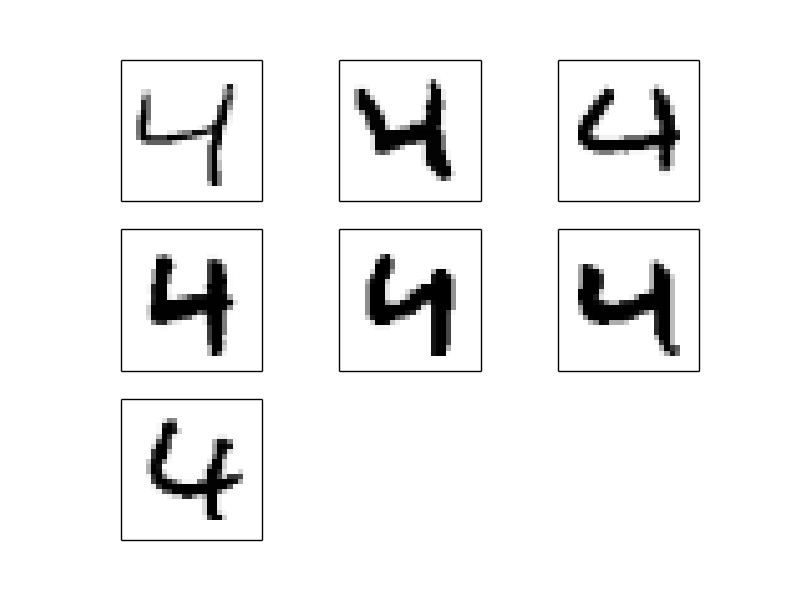
\includegraphics[scale=0.5]{meansA2}
\caption{Digits 2}
\end{center}
\end{figure}
\begin{figure}
\begin{center}
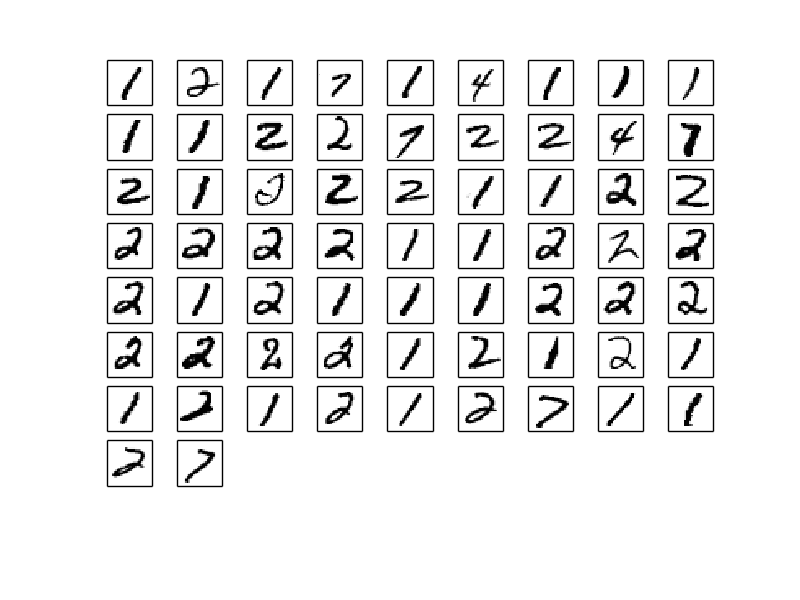
\includegraphics[scale=0.5]{meansA3}
\caption{Digits 3}
\end{center}
\end{figure}
\begin{figure}
\begin{center}
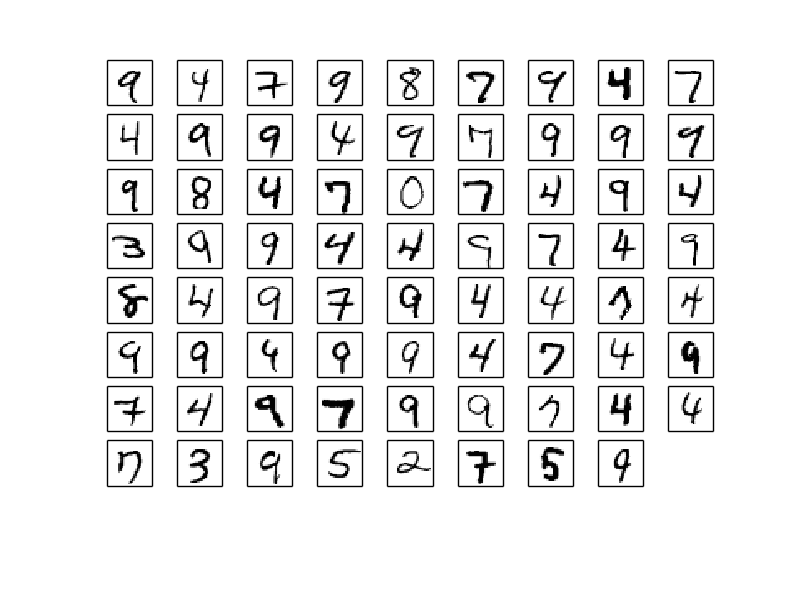
\includegraphics[scale=0.5]{meansA4}
\caption{Digits 4}
\end{center}
\end{figure}
\begin{figure}
\begin{center}
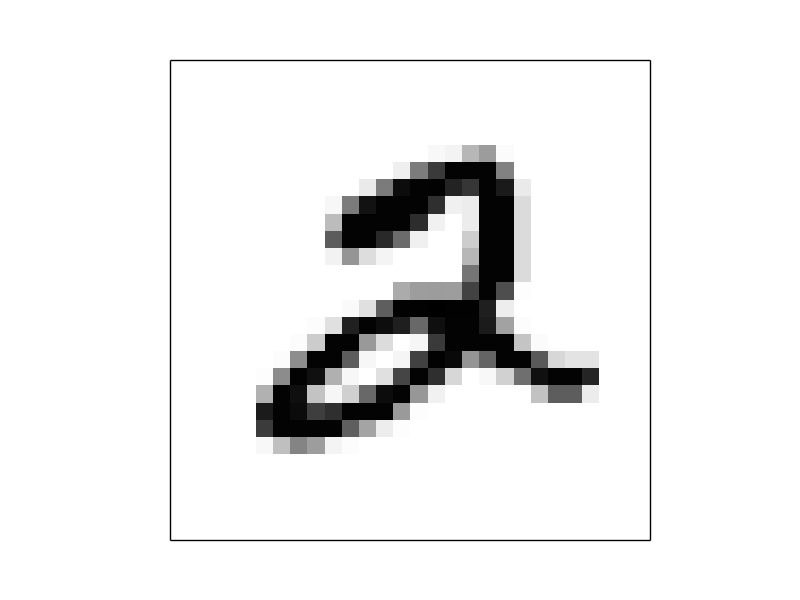
\includegraphics[scale=0.5]{meansA5}
\caption{Digits 5}
\end{center}
\end{figure}
\begin{figure}
\begin{center}
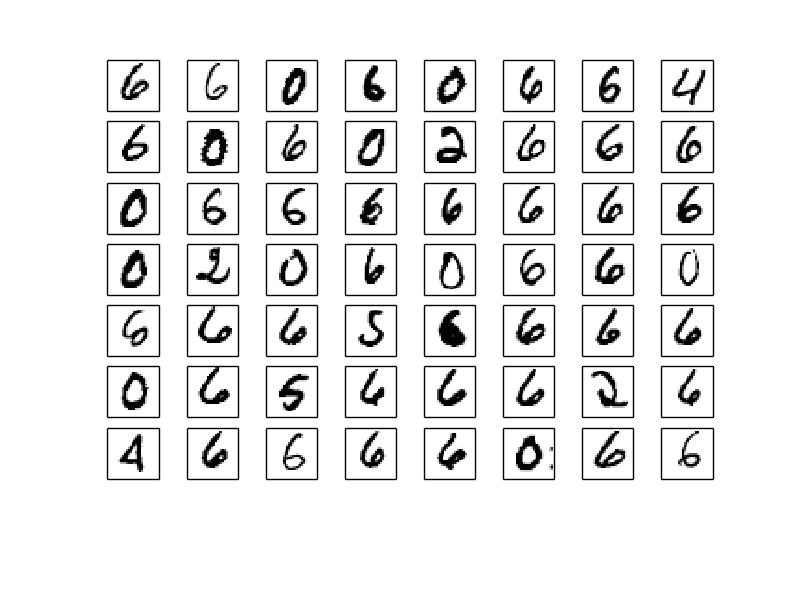
\includegraphics[scale=0.5]{meansA6}
\caption{Digits 6}
\end{center}
\end{figure}
\begin{figure}
\begin{center}
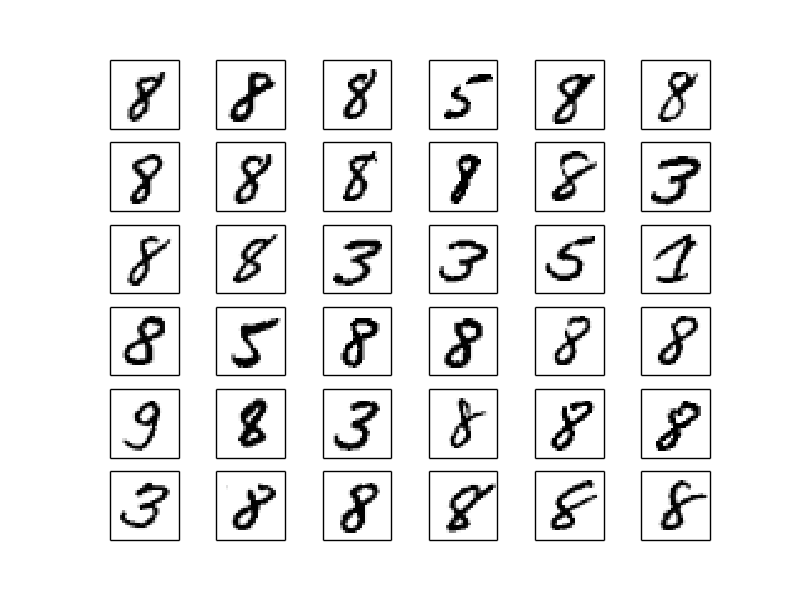
\includegraphics[scale=0.5]{meansA7}
\caption{Digits 7}
\end{center}
\end{figure}
\begin{figure}
\begin{center}
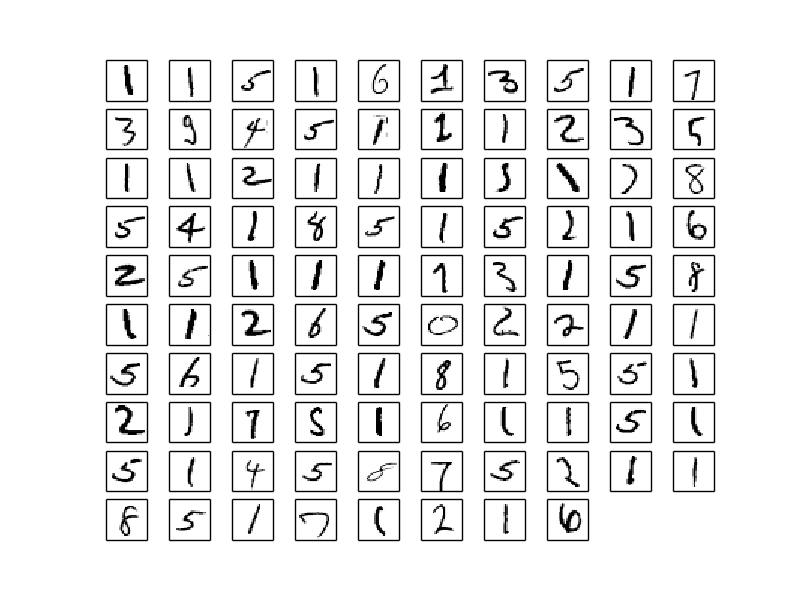
\includegraphics[scale=0.5]{meansA8}
\caption{Digits 8}
\end{center}
\end{figure}
\begin{figure}
\begin{center}
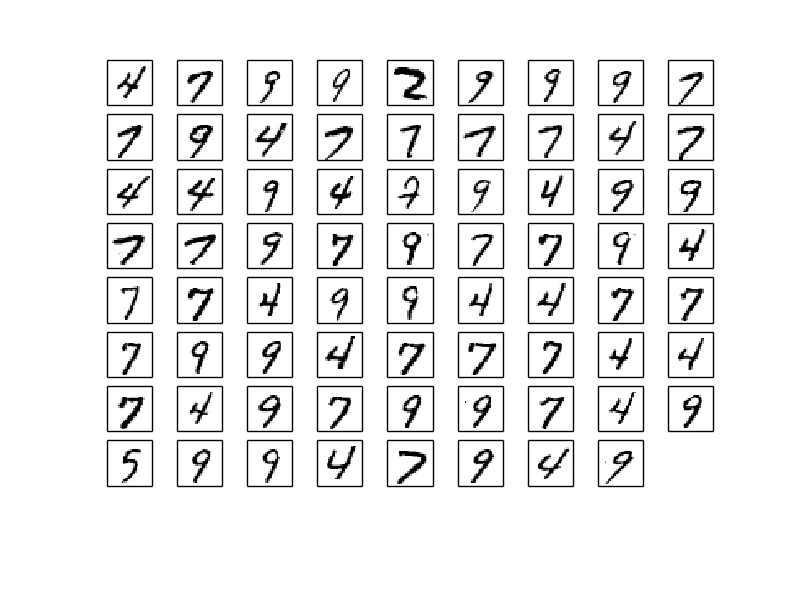
\includegraphics[scale=0.5]{meansA9}
\caption{Digits 9}
\end{center}
\end{figure}

\clearpage

\subsubsection{Use the first images with \textbf{distinct} digits}
Here, we used the first 10 \textbf{unique} digits as the initial cluster means.
\begin{figure}[H]
\begin{center}
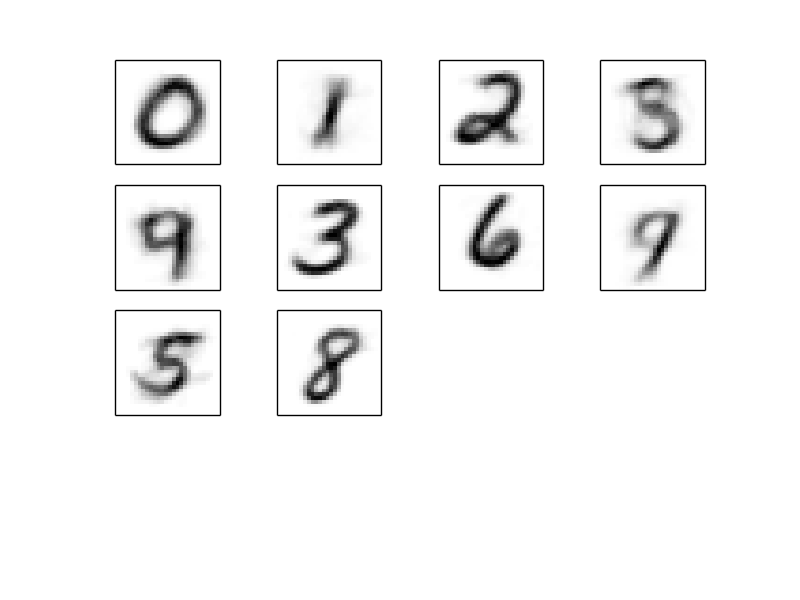
\includegraphics[scale=0.5]{meansB}
\caption{Second iteration cluster means}
\end{center}
\end{figure}
The classified digits follow:
\begin{figure}
\begin{center}
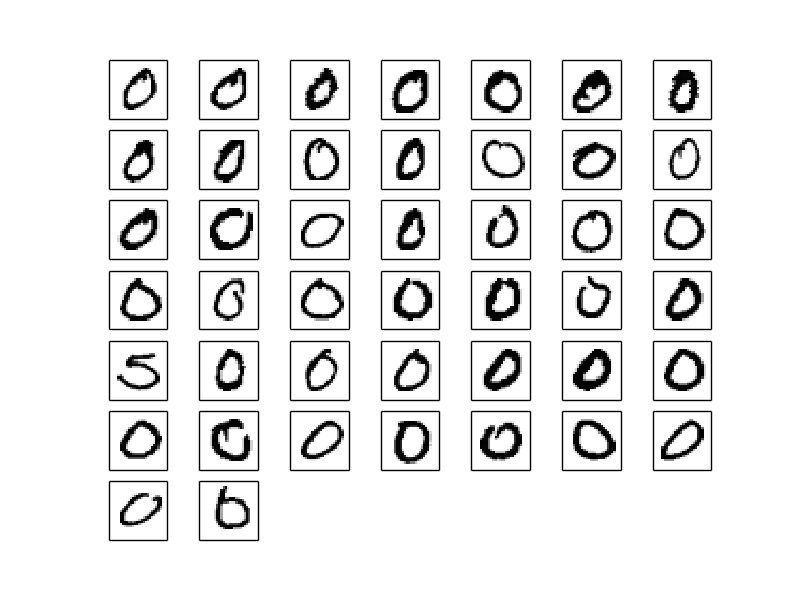
\includegraphics[scale=0.5]{meansB0}
\caption{Digits 0}
\end{center}
\end{figure}
\begin{figure}
\begin{center}
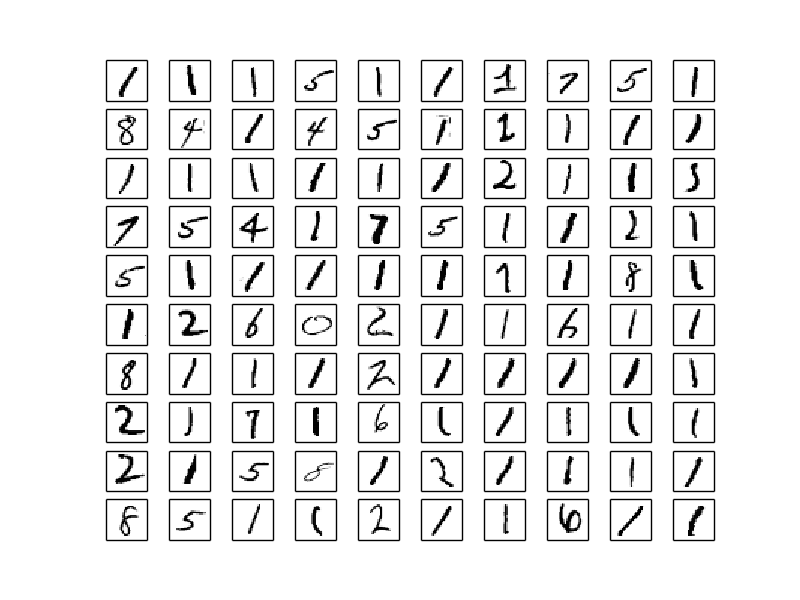
\includegraphics[scale=0.5]{meansB1}
\caption{Digits 1}
\end{center}
\end{figure}
\begin{figure}
\begin{center}
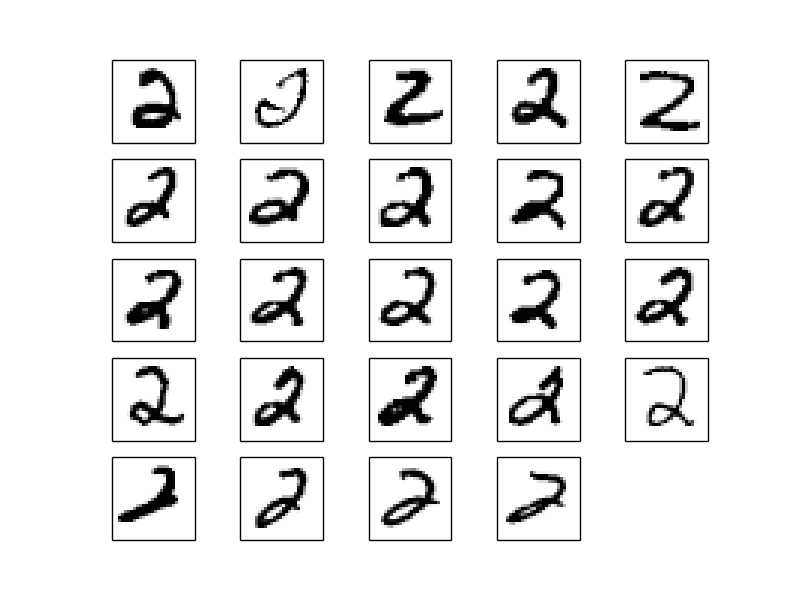
\includegraphics[scale=0.5]{meansB2}
\caption{Digits 2}
\end{center}
\end{figure}
\begin{figure}
\begin{center}
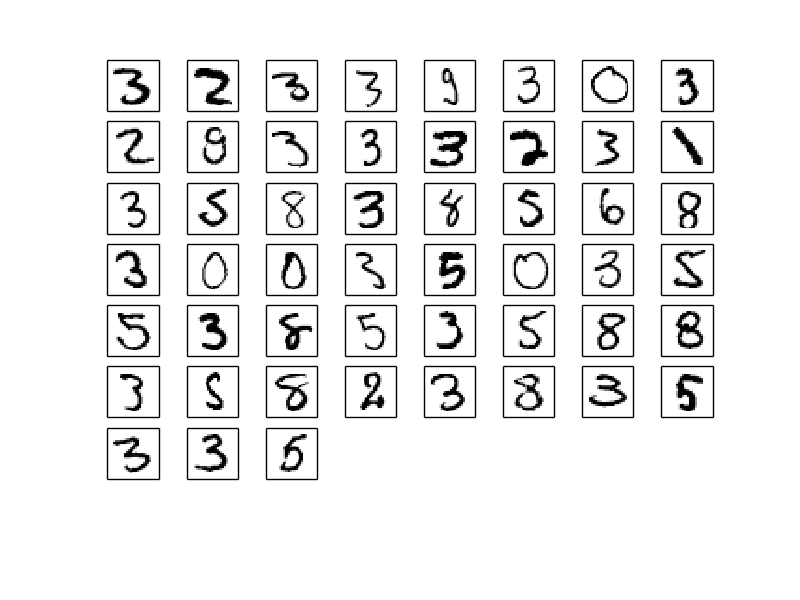
\includegraphics[scale=0.5]{meansB3}
\caption{Digits 3}
\end{center}
\end{figure}
\begin{figure}
\begin{center}
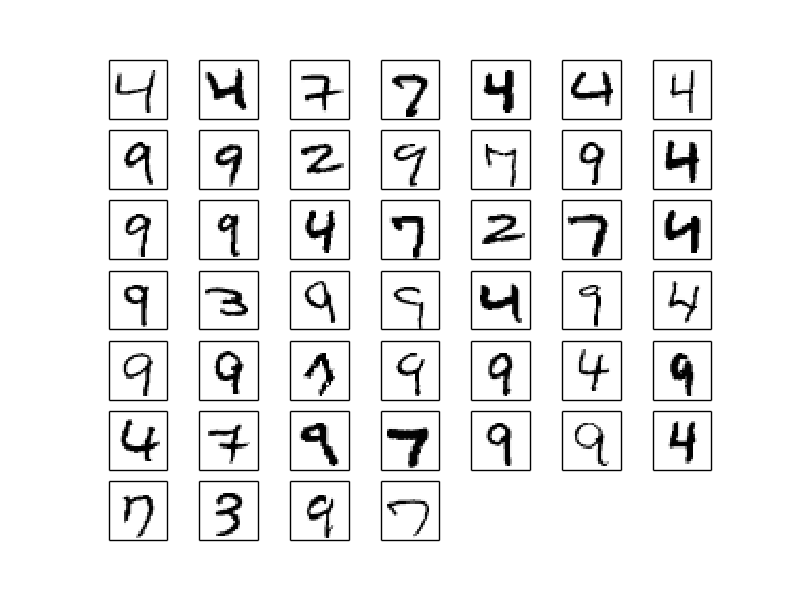
\includegraphics[scale=0.5]{meansB4}
\caption{Digits 4}
\end{center}
\end{figure}
\begin{figure}
\begin{center}
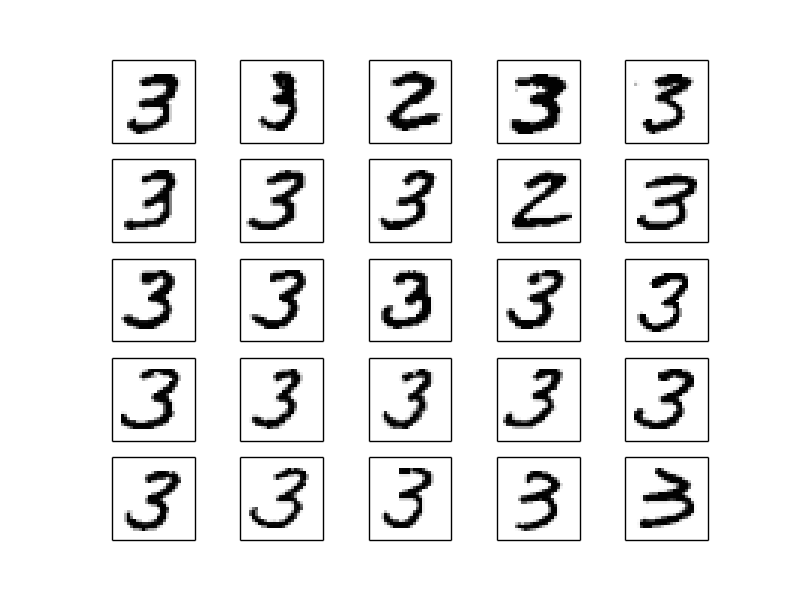
\includegraphics[scale=0.5]{meansB5}
\caption{Digits 5}
\end{center}
\end{figure}
\begin{figure}
\begin{center}
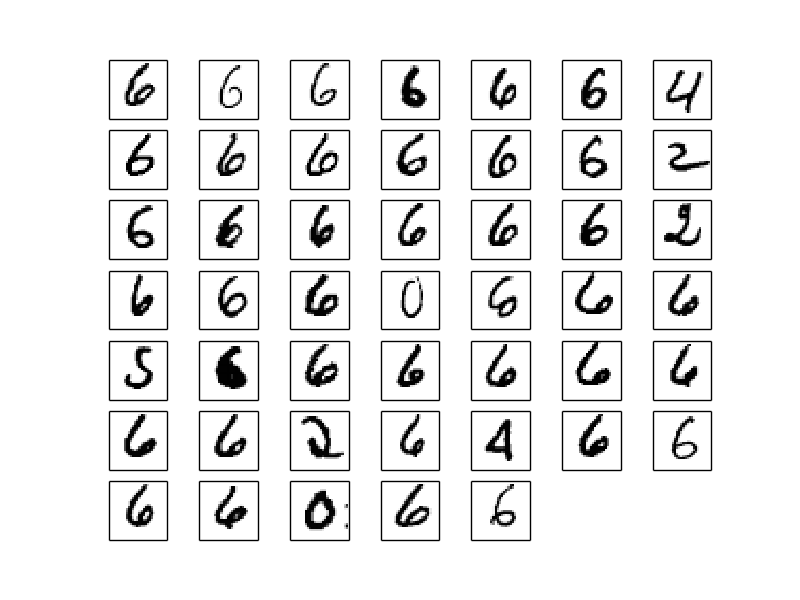
\includegraphics[scale=0.5]{meansB6}
\caption{Digits 6}
\end{center}
\end{figure}

\begin{figure}
\begin{center}
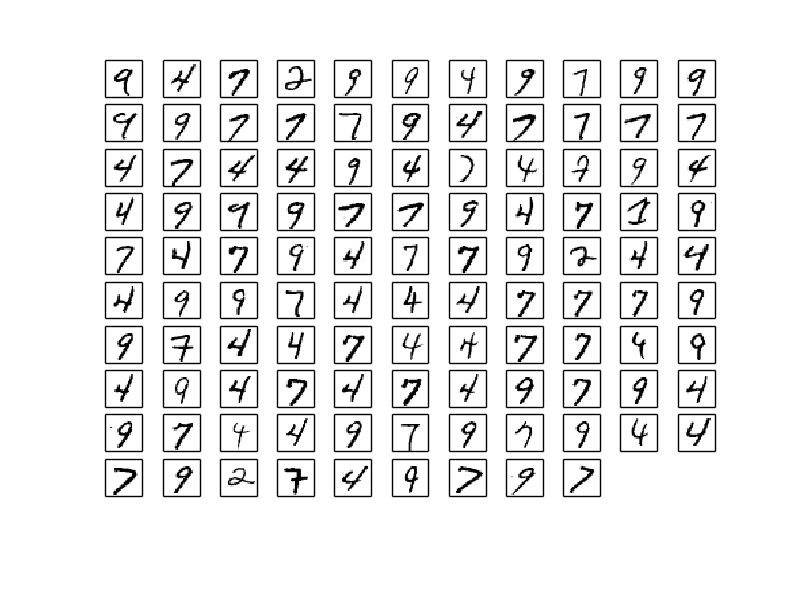
\includegraphics[scale=0.5]{meansB7}
\caption{Digits 7}
\end{center}
\end{figure}
\begin{figure}
\begin{center}
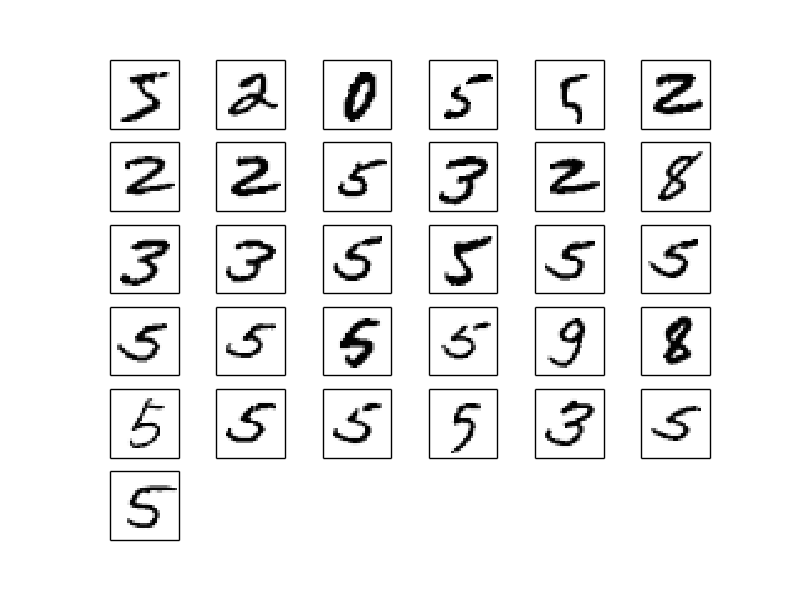
\includegraphics[scale=0.5]{meansB8}
\caption{Digits 8}
\end{center}
\end{figure}
\begin{figure}
\begin{center}
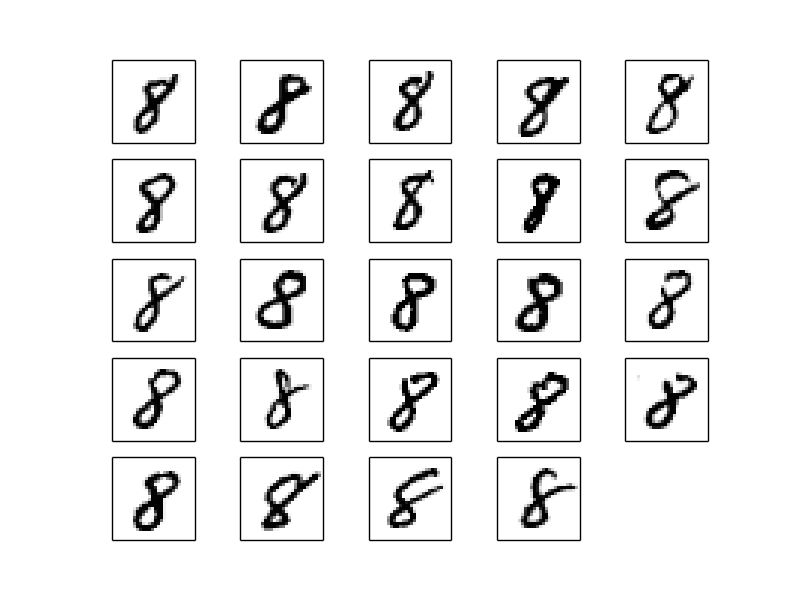
\includegraphics[scale=0.5]{meansB9}
\caption{Digits 9}
\end{center}
\end{figure}
Obvously, the first iteration with non-unique digits as the initial cluster means perform rather poorly. The second iteration that uses distinct digit clusters improves on the latter, yet it is far from perfect.

\end{document}